\documentclass[11pt]{article}

\usepackage[utf8]{inputenc}
\usepackage[T1]{fontenc}
\usepackage[french]{babel}
\usepackage{graphicx}
\usepackage[a4paper,left=2.5cm,right=2cm,top=2.5cm,bottom=2.5cm]{geometry}
\usepackage{csquotes}
\usepackage{hyperref}

\graphicspath{{res/}}

\begin{document}


\includegraphics[width=\linewidth]{certificat.png}

\bigskip

Félicitations ! Pendant une heure, vous avez appris et mis en pratique des concepts fondamentaux en informatique !

\bigskip

Vous avez notamment appris : \newline

\begin{center}
\begin{tabular}{|c|c|}
    \hline
    \textbf{L'exécution séquentielle} & \textbf{Les boucles} \\
     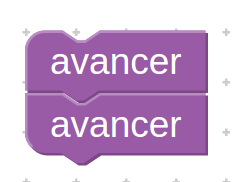
\includegraphics[width=0.15\linewidth]{blocks_2moveForward.png} &
     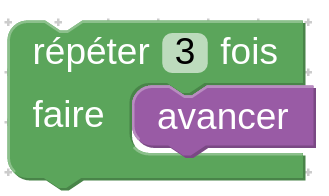
\includegraphics[width=0.2\linewidth]{blocks_forloop.png} \\
   \hline
   \textbf{Les conditions} & \textbf{Les fonctions} \\
   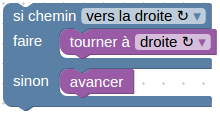
\includegraphics[width=0.3\linewidth]{blocks_ifElse.png} &
   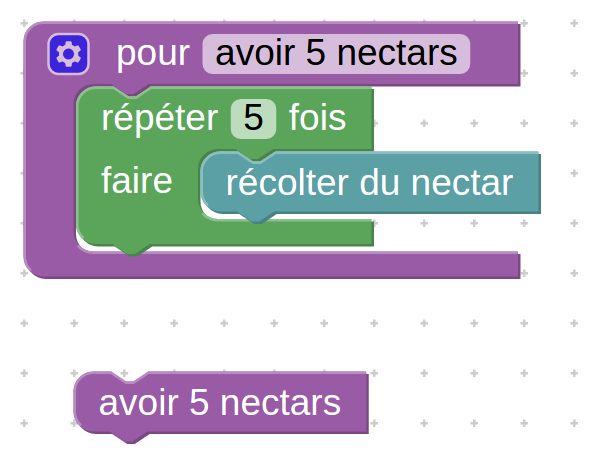
\includegraphics[width=0.3\linewidth]{blocks_function.png} \\
   \hline
\end{tabular}
\end{center}

\bigskip

Vous êtes maintenant familier avec l'interface de blocs \enquote{Blockly} !

\bigskip

Vous souhaitez en apprendre encore plus ? Rendez-vous sur \url{https://code.org/learn}

\bigskip

Vous pourrez \textbf{créer des jeux} et résoudre des problèmes avec \textbf{Minecraft, Flappy Bird, Star Wars, La Reine des Neiges, Angry Birds}
et plein d'autres jeux !

\end{document}
